\section{Introduction}
Online tools increasingly rely on large amounts of data collected from the crowd.
For example, user-submitted product ratings in an e-commerce site can help recommend products to similar users in the future.
Rating data, like traditional surveys, are subject to a variety of biasing tendencies \cite{groves2013survey}.
We explore a class of biases, collectively called \emph{Social Influence Bias}, which arise from feedback from the actions of other users in the system \cite{demarzo2003persuasion, moscovici1972social, wood2000attitude}.
One aspect of Social Influence Bias is the phenomenon called \emph{social herding}, where the feedback from the community encourages future participants to conform to what they perceive as the ``norm" in the community.
The effects of social herding are crucial to the design of recommendation algorithms as many algorithms assume statistical independence between different users and use the spatial relationships between numerical features representing those users.

\begin{figure}[h]
  \centering
    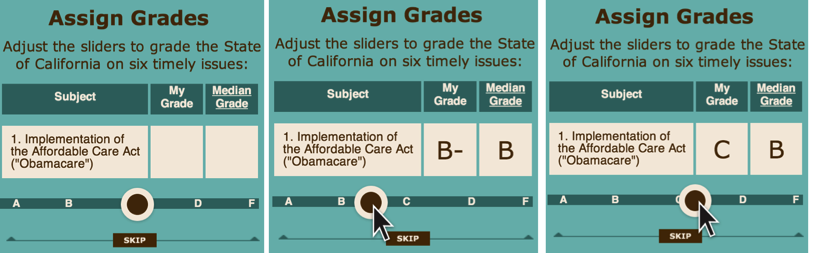
\includegraphics[width=\columnwidth]{../plots/grading-desc-1.png}
      \caption{Grading in the California Report Card. Participants enter grades on six timely issues facing the State of California. After entering their grades, the median grade over all participants is revealed. Participants have the option to change their grades after seeing the median. We model the tendency to regress towards the medians.}
      \label{grading-1}
\end{figure}

A common feedback mechanism is the use of aggregate statistics, for example, showing the average rating for a product before a participant shares his or her rating (Figure \ref{grading-1}).
In recent related work, Muchnik et al. \cite{muchnik2013social}, used a randomized experiment to determine the magnitude of social herding in up-voting in Reddit.com.
They randomly treated forum posts with extra up-votes and down-votes and measured the treatment effect; concluding that a statistically significant social herding tendency exists.
In this paper, we explore a related problem of whether users who have already submitted a rating will actually \emph{change} their existing ratings upon learning the median rating for the population and ``herd" towards the median grade.

As a case study, we use data from the California Report Card (CRC) \cite{crc}, where users graded the state of California on six timely issues.
After submitting a grade, users were shown the median grade of all other users.
We recorded any changes to previous grade that happened after the median was visible.
Such feedback of social content is an established technique to incentivize participation and increase user engagement with the tool \cite{shneiderman1992designing}.  
Furthermore, an application of particular interest is online participatory democracy where open aggregate results increase the transparency of the system \cite{albors2008new,o2012transparency,noveck2008wiki}.
For comparision with the CRC, we ran a reference survey through SurveyMonkey which was given to a random 611 participants from the company's paid pool of California participants.
In this survey, we asked users to respond to the same questions as the CRC on the same grading scale without the feedback of the median grade. 

The findings of Muchnik et al. suggest that social herding will be observed in the form of a regression towards the observed median grade during the grade changes.
In this paper, we test the hypothesis of social herding, propose a model for the relationship between observed medians and subsequent grade change, and provide experimental results comparing the data from the CRC to the randomized reference survey.

\subsection{Hypotheses and Contributions}
\noindent \textbf{Null Hypothesis} Viewing the median grade does not affect how a user chooses to change his or her grade, and does not affect any future grades given by the participant.

\noindent \textbf{Social Herding Around the Median} Grade changes are on average towards the median grade. Also, the final grades of participants who change their grades are more tightly concentrated around the median from participants who did not change their grades and participants from the reference survey.

\noindent \textbf{Social Herding and Question Order} Disagreement with the median on previous questions affect how a participant grades future questions. Participants who disagreed with the median greatly are more likely to leave future responses that are closer to the median. 

We develop non-parametric testing procedure, based on the Wilcoxon Rank-Sum statistic (also called the Mann-Whitney statistic) \cite{lehmann2006nonparametrics}, to test these hypotheses.
We chose a non-parametric framework because Muchnik et al. focused on only a binary input mechanism (up or down vote) and we extended this analysis to grading sliders with 13 possible vales from (A+ to F) without having to make strong assumptions about the distribution of grades.
In addition to the hypothesis testing, we model grade changes with a polynomial regression.
As before, to avoid having to make a strong assumption about the structure of the model, we use an information theoretic model to learn a flexibile degree polynomial.

